\documentclass[12pt]{article}
\usepackage[utf8]{inputenc}
\usepackage{geometry}
\geometry{margin=1in}
\usepackage{graphicx, amsmath}
\usepackage{tikz}
\usepackage{multicol}
\usepackage{circuitikz}
\setlength{\parindent}{0in}

\title{Physics review sheet}
\author{Simon Wu }
\date{February 2021}

\begin{document}
\maketitle

\tableofcontents

%\Large{Lens Formulas}\\
%\large

\newpage

%\section{Mirrors}

%\section{Interference}

%\subsection{Single-slit diffraction}

%\subsection{Double-slit diffraction}

%\section{Electricity}

%\subsection{Capacitors}

%\subsection{Conducting spheres}

%\subsection{Non-conducting spheres}

\section{Optics}

\subsection{Lensmaker's formula}

Given an object distance $p$, image distance $q$ and focal length $f$:

\[
\boxed{\frac{1}{f} = \frac{1}{p} + \frac{1}{q}}
\]\\

\begin{multicols}{2}

\subsection{Lens types}
\small

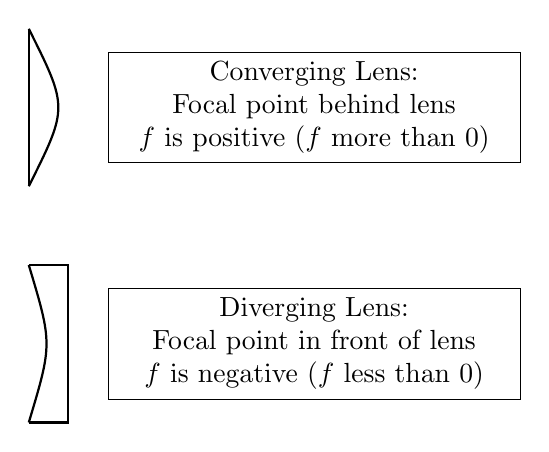
\begin{tikzpicture}
%\draw[step=1cm,gray,very thin] (-2,-2) grid (10,10);

\draw[thick](0,3) -- (0,5);
\draw[thick](0,3) .. controls (0.5,4) .. (0,5);

\node[draw, anchor=west, align=center, text width=5cm] at (1,4) {Converging Lens:\\ Focal point behind lens\\ $f$ is positive ($f$ more than 0)};

\draw[thick](0,0) -- (0.5,0) -- (0.5,2) -- (0,2);
\draw[thick](0,0) .. controls (0.3,1) .. (0,2);

\node[draw, anchor=west, align=center, text width=5cm] at (1,1) {Diverging Lens:\\ Focal point in front of lens\\ $f$ is negative ($f$ less than 0)};

\end{tikzpicture}
\columnbreak

\subsection{Sign convention}
\begin{center}
\begin{tabular}{ |c|c|c| } 
 \hline
  & Front of lens & Behind lens \\ 
  \hline
 f & Negative (-) & Positive (+) \\ 
 \hline
 p & Positive (+) & Negative (-) \\ 
 \hline
 q & Negative (-) & Positive (+) \\
 \hline
\end{tabular}
\end{center}
\end{multicols}

\subsection{Combining lenses}
\begin{center}
\small
\begin{tikzpicture}
%\draw[step=1cm,gray,very thin] (0,0) grid (14,6);

\draw[thick,->](1,3) -- (1,4);

\node[anchor=south, align=center] at (2.5,4) {$p_1$};

\draw[thick,<->](1,4) -- (4,4);

\filldraw (1,4) circle (2pt);

\draw[thick](4,1) rectangle (5,5);

\node[anchor=north, align=center] at (4.5,1) {$f_1$};

\draw[thick](10,1) rectangle (11,5);

\node[anchor=north, align=center] at (10.5,1) {$f_2$};

\draw[thick,<->](5,5) -- (10,5);

\node[anchor=south, align=center] at (7.5,5) {$d$};

\draw[thick,<->](11,4) -- (13,4);

\draw[thick,<->](5,2) -- (7,2);
\node[anchor=north, align=center] at (6,2) {$q_1$};
\draw[thick,<->](7,2) -- (10,2);
\node[anchor=north, align=center] at (8.5,2) {$p_2$};

\filldraw (13,4) circle (2pt);

\draw[thick,->](13,3) -- (13,4);

\node[anchor=south, align=center] at (12,4) {$q_2$};

\draw[thick,dashed](0,3) -- (14,3);

\end{tikzpicture}

\end{center}

\begin{multicols}{2}
{
%\begin{center}
\subsubsection{Working with multiple lenses}
\[
\boxed{\frac{1}{d-q_1}+\frac{1}{q_2}=\frac{1}{f_2}}
\]
%\end{center}
}

\columnbreak

%\begin{center}
\subsubsection{As $d\longrightarrow 0$}

\[
\boxed{\frac{1}{f_{\text{eff}}}=\frac{1}{f_1}+\frac{1}{f_2}}
\]

Two lenses stuck together ($d \approx 0$) may be treated as a single lens with a new effective focal length $f_{\text{eff}}$.
%\end{center}

\end{multicols}

\subsection{Magnification}

Linear magnification is based on the object and image distances $p$ and $q$:

\[
\boxed{
M = \frac{h'}{h} = -\frac{q}{p}
}
\]

If $h' < 0$, the image is inverted.

\subsection{Polarization}

The intensity of light passing through a polarizing sheet is one half of the intensity of the light incident to the sheet:

\[
\boxed{
I' = \frac{I}{2}
}
\]

\subsubsection{Malus' law}

If the light then passes through another polaroid that is at an angle $\theta$ to the first polaroid, then the intensity it related to the square of the cosine of the angle:

\[
\boxed{
I'' = \frac{I}{2}\cos^2 (\theta)
}
\]

\subsection{Double slit interference}

\subsubsection{Bright fringes}

Bright fringes on the screen are evenly spaced.
Given wavelength of light $\lambda$, width of gap between slits $d$ and distance from screen $L$:

\[
\boxed{
y_n = \frac{n\lambda L}{d}
}
\]

$n$ is an integer ($1, 2, 3 ...$)

\subsubsection{Bright fringes}

Dark fringes on the screen are also evenly spaced.
Given wavelength of light $\lambda$, width of gap between slits $d$ and distance from screen $L$:

\[
\boxed{
y_n = \left(n + \frac{1}{2}\right)\frac{\lambda L}{d}
}
\]

$n$ is an integer ($1, 2, 3 ...$)

\newpage

\subsection{Single slit interference (diffraction)}

Diffraction is the rounding of a wavefront as it moves through a small opening, especially an opening that is much smaller than its wavelength.

\begin{center}

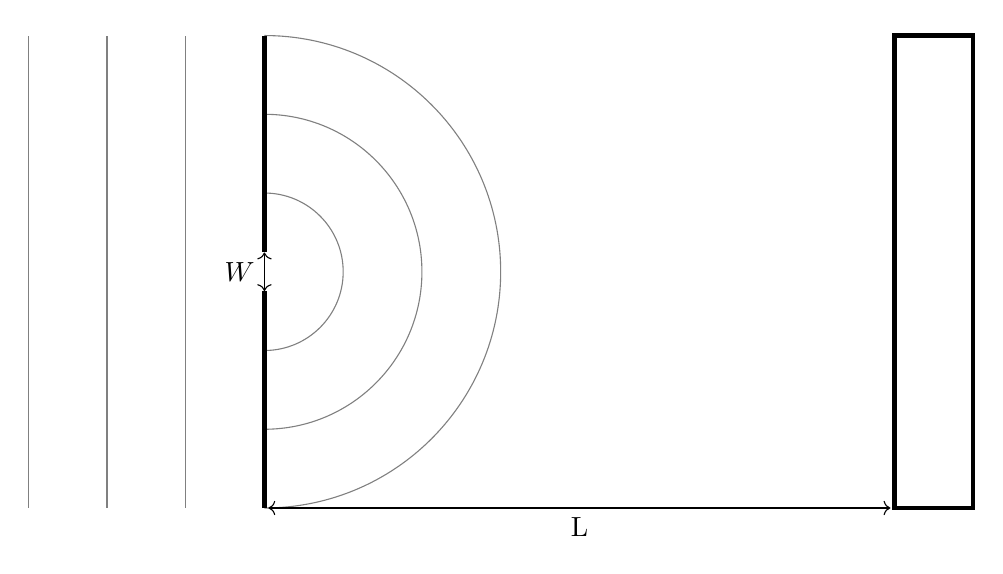
\begin{tikzpicture}

\draw[gray, thin] (-3,-3) -- (-3,3);

\draw[gray, thin] (-2,-3) -- (-2,3);

\draw[gray, thin] (-1,-3) -- (-1,3);

\begin{scope}
    \clip (0,-1.1) rectangle (1.1,1.1);
    \draw[gray, thin] (0,0) circle(1);
\end{scope}

\begin{scope}
    \clip (0,-2.1) rectangle (2.1,2.1);
    \draw[gray, thin] (0,0) circle(2);
\end{scope}

\begin{scope}
    \clip (0,-3.1) rectangle (3.1,3.1);
    \draw[gray, thin] (0,0) circle(3);
\end{scope}

\draw[thin, <->] (0, -0.245) -- (0, 0.245);

\node[anchor=east] (0,0) {$W$};

\draw[black, ultra thick] (0,3) -- (0,0.25);

\draw[black, ultra thick] (0,-3) -- (0,-0.25);

\draw[thin, <->] (0.05, -3) -- (7.95, -3);

%\node[anchor=east] (4,-3) {$L$};

\draw[black] (4, -3) node[anchor=north] {L};

\draw[ultra thick] (8, -3) rectangle (9, 3);

\end{tikzpicture}

\end{center}

\subsubsection{Bright fringes}

Bright fringes on the screen are evenly spaced.
Given wavelength of light $\lambda$, width of gap $W$ and distance from screen $L$:

\[
\boxed{
y_m = \left(m + \frac{1}{2}\right)\frac{\lambda L}{W}
}
\]

$m$ is an integer ($1, 2, 3 ...$)

\subsubsection{Dark fringes}

Dark fringes on the screen are also evenly spaced, and between the light fringes.
Given wavelength of light $\lambda$, width of gap $W$ and distance from screen $L$:

\[
\boxed{
y_m = \frac{m\lambda L}{W}
}
\]

Notice that the pattern is very similar to the double-slit interference pattern, but reversed between the dark and bright fringes.

\newpage

\subsection{Thin-film interference}

\newpage

\section{Electricity}

\subsection{Current}

Conventional current is the rate at which positive charges flow through a wire:

\[
\boxed{
I = \frac{\mathrm{d}Q}{\mathrm{d}t}
}
\]

It is also defined as the flux of charge density flowing past a surface (like the cross-section of a wire):

\[
\boxed{
I = \int \vec{J} \cdot \mathrm{d}\vec{A}
}
\]

\subsection{Resistors}

\subsubsection{Resistivity}

Resistivity of a material is proportional to the electric field and current density:

\[
\boxed{
\vec{E} = \rho \vec{J}
}
\]

Electric field is in newtons per coulomb, charge density in amperes per meter squared, and resistivity in ohms per meter.

\subsubsection{Resistance of a conductor}

Resistance of a conductor is proportional to resistivity $\rho$ and length $L$ and inversely proportional to cross-sectional area $A$:

\[
\boxed{
R = \rho \frac{L}{A}
}
\]

\subsubsection{Power dissipated by a resistor}

The power $P$ dissipated by a resistor of resistance $R$, given a potential difference $V$ and a current $I$ across the resistor:

\[
\boxed{
P = IV = \frac{V^2}{R} = I^2 R
}
\]

\subsubsection{Resistors in parallel}

The equivalent resistance $R_{eq}$, given $N$ resistors with resistances $R_1$, $R_2$ ... $R_N$ in parallel:

\[
\boxed{
\frac{1}{R_{eq}} = \frac{1}{R_1} + \frac{1}{R_2} + ... \frac{1}{R_N}
}
\]

\newpage

\subsubsection{Resistors in series}

The equivalent resistance $R_{eq}$, given $N$ resistors with resistances $R_1$, $R_2$ ... $R_N$ in series:

\[
\boxed{
R_{eq} = R_1 + R_2 + ... + R_N
}
\]

\subsection{Capacitors}

A parallel-plat capacitor creates a potential difference between 2 plates by transferring changes between the plates when connected to a battery.
This stores energy in the capacitor that can be used later.

\subsubsection{Capacitance}

The plates of a capacitor will develop a charge of $Q$ and $-Q$.
The relation between the charge on the plates and the potential difference is the capacitance:

\[
\boxed{
C = \frac{Q}{\Delta V}
}\text{ or }
\boxed{Q = C \Delta V}
\]

The units of capacitance are farads, which are coulombs per volt. $(F = C/V)$

If the potential difference is considered in terms of the electric field $E$ and distance $d$ between the plates, and the charge is considered in terms of charge density $\sigma$ and area $A$ of the plates:

\[
\boxed{
C = \frac{\sigma A}{Ed} = \frac{\sigma A}{(\sigma / \epsilon_0) d} =\epsilon_0 \frac{A}{d}
}
\]

\subsubsection{Energy stored in a capacitor}

Given that a capacitor has a potential difference $V$ across it and is storing $Q$:

\[
\boxed{
U_c = \frac{1}{2}\frac{Q^2}{C} = \frac{1}{2}QV = \frac{1}{2}CV^2
}
\]

\subsubsection{Dielectric materials}

A dielectric reduces the electric field within it by a factor of $\kappa$:

\[
\boxed{
\kappa = \frac{E_0}{E}
}
\]

It can also be viewed as increasing effective permittivity:

\[
\boxed{
\epsilon = \kappa \epsilon_0
}
\]

Dielectric materials amplify capacitance by a factor of $\kappa$:

\[
\boxed{
C = \kappa C_0
}
\]

\newpage

\subsubsection{Capacitors in parallel}

The potential difference across capacitors in parallel will be the same.
The equivalent capacitance $C_{\text{eq}}$, given $N$ capacitors $C_1, C_2, ... C_N$ in parallel:

\[
\boxed{
C_{\text{eq}} = C_1 + C_2 + ... + C_N
}
\]

\subsubsection{Capacitors in series}

The total voltage (potential difference) across capacitors in series must be the sum of the voltages across each of them.
The charges stored in each of the capacitors must also be the same!
From this, given $N$ capacitors $C_1, C_2, ... C_N$ in series:

\[
\boxed{
\frac{1}{C_{\text{eq}}} = \frac{1}{C_1} + \frac{1}{C_2} + ... + \frac{1}{C_N}
}
\]

\subsubsection{Discharging a capacitor}

\begin{center}
\begin{circuitikz} \draw
(0,0) to (2,0) to[ capacitor, l=$C$] (2,-2) to (0, -2) to[ american resistor, l=$R$ ] (0,0); 
\end{circuitikz}
\end{center}

Considering a capacitor charged to $V_c = Q_{\text{tot}}/C$ and a capacitor $R$: as current flows, the charge on the capacitor decreases, and the current decreases, until the capacitor is fully discharged and the current stops flowing. We can apply Kirchhoff's Voltage Law:

\[
\boxed{V_c - IR = 0} \rightarrow \boxed{-\frac{Q}{C} - R\frac{\mathrm{d}Q}{\mathrm{d}t} = 0} \rightarrow \boxed{\frac{\mathrm{d}q}{\mathrm{d}Q} = -\frac{\mathrm{d}t}{RC}}
\]

Solving that differential equation, you obtain the expression of charge across the capacitor, which is time-dependent:

\[
\boxed{
Q(t) = Q_0 e^{-t/\tau}
}
\]

$Q_0$ is the initial capacitor change $Q_{\text{tot}}$, and $\tau = RC$, which is called the time constant.
Taking the derivative of $Q(t)$ to derive the current through the circuit:

\[
\boxed{
I(t) = \frac{\mathrm{d}Q}{\mathrm{d}t} = I_0 e^{-t/\tau}
}
\]

$I_0$ is the initial current at $t=0$.
It is given by $Q_{\text{tot}}/\tau = Q_{\text{tot}}/RC$.

\newpage

\subsubsection{Charging a capacitor}

\begin{center}
\begin{circuitikz} \draw
(0,0) to[ american resistor, l=$R$ ] (2,0) to[ capacitor, l=$C$] (2,-2) to (0, -2) to[ battery, l=$V$ ] (0,0); 
\end{circuitikz}
\end{center}

Now, consider the case where there is now a battery in the circuit. We can again apply Kirchhoff's Voltage Law:

\[
\boxed{V - R\frac{\mathrm{d}Q}{\mathrm{d}t} - \frac{Q}{C} = 0} \rightarrow \boxed{ \frac{\mathrm{d}Q}{CV - Q} = -\frac{\mathrm{d}t}{RC}}
\]

Integrating and then exponentiating:

\[
\boxed{CV - Q = e^K e^{-t/RC}}
\]

When $t = 0$, charge across the capacitor $Q$ is also $0$:

\[
\boxed{e^K = CV = Q_{\text{tot}}}
\]

Therefore, we can find that the charge across the capacitor is time-dependent again:

\[
\boxed{ Q(t) = Q_{\text{tot}}(1 - e^{-t/\tau}) }
\]

Once again, we can differentiate to find the current through the circuit, which is actually identical to when it is discharging:

\[
\boxed{ I(t) = \frac{\mathrm{d}Q}{\mathrm{d}t} = I_0 e^{-t/ \tau} }
\]

The time constant $\tau$ is the same as when the capacitor is being discharged.
Initial current $I_0$ is given by $Q_{\text{tot}}/\tau = V/R$, which makes sense.

\subsection{Inductors}

\newpage

\section{Magnetism}

\subsection{Lorentz force law}

The force acting on a charged particle $q$ in an electric field $\vec{E}$ and magnetic field $\vec{B}$ and moving with velocity $\vec{v}$:

\[
\boxed{\vec{F} = q\left(\vec{E} + \vec{v} \times \vec{B}\right)}
\]

\subsection{Magnetic flux}

Magnetic flux through a wire loop of area $\vec{A}$ in a field $\vec{B}$ that is making an angle $\theta$ perpendicular to the loop, in units of weber:

\[
\boxed{
\phi_B = \int \vec{B} \cdot \mathrm{d}\vec{A}
}
\]

Simplifies when the magnetic field is constant over the area of the wire loop:

\[
\boxed{
\phi_B = \vec{B} \cdot \vec{A}
}
\]

\[
\boxed{
\phi_B = BA\cos(\theta)
}
\]

\subsubsection{Faraday's law}

Faraday's law states that electromotive force is inducted in a conductor when there is a change in the number of field lines passing through it, or when it cuts across field lines. The electromotive force $\varepsilon$ induced in a wire loop is the rate of change of flux through it.

\[
\boxed{
\varepsilon = -\frac{\mathrm{d}\phi_B}{\mathrm{d}t} = -\frac{\Delta \phi_B}{\Delta t}
}
\]

\subsubsection{Lenz's law}

Lenz's law states that induced current will appear in such a direction that it opposes the charge that produced it.
For example, if the area of a loop of wire in a magnetic field coming out of the page is decreasing, the magnetic flux through the loop is decreasing: induced current will appear such that it counteracts that decrease, indicating that the current will be counterclockwise (inducing more field out of the page inside the loop).

\subsubsection{Electromotive force in a coil}

Given a coil of $N$ turns:

\[
\boxed{
\varepsilon=-N\frac{\Delta \phi_B}{\Delta t}
}
\]

\newpage

\subsection{Magnetic induction from a current in a wire}

\subsubsection{Magnetic field at the centre of a coil}

Given a coil of $N$ turns, radius $r$ and carrying current $i$:

\[
\boxed{
B=\frac{\mu_0 Ni}{2r}
}
\]

\subsubsection{Magnetic field on the axis of a solenoid}

Given a solenoid of $N$ turns over an axial length $l$:

\[
\boxed{
B = \frac{\mu_0 Ni}{l}
}
\]

\subsubsection{Magnetic field from a straight wire}

At a distance $r$ from a wire carrying current $i$, with the position subtending angles $\theta_1$ and $\theta_2$ from the ends of the wire"

\[
\boxed{
B = \frac{\mu_0 i}{4\pi r}\left(\cos(\theta_1) + \cos(\theta_2)\right)
}
\]

\subsubsection{Magnetic field from an infinitely long wire}

Given that our wire is now infinitely long, meaning that $\theta_1 \longrightarrow 0$ and $\theta_2 \longrightarrow 0$:

\[
\boxed{
B = \frac{\mu_0 i}{2\pi r}
}
\]

\subsection{Cyclotron concepts}

\subsubsection{Radius of motion of a particle in a magnetic field}

Assuming that a field $B$ acts perpendicularly to the plane of orbit of a particle $q$ and mass $m$ moving with velocity $v$:

\[
\boxed{
r = \frac{mv}{qB}
}
\]\\

\begin{multicols}{2}

\subsubsection{Angular frequency}

\[
\boxed{
\omega = \frac{v}{r}=\frac{qB}{m}
}
\]

\columnbreak

\subsubsection{Cyclotron frequency}

\[
\boxed{
f = \frac{\omega}{2\pi}=\frac{qB}{2\pi m}
}
\]

\end{multicols}

%\section{Inducers}

\newpage

\section{Special relativity}

\subsection{Rapidity}

Given a a frame of reference that moves at a velocity $v$, and a variable $\beta$ defined as $\frac{v}{c}$, and where $\zeta$ is the rapidity:

\[
\boxed{
\tanh(\zeta) = \beta
}
\]

\subsubsection{Hyperbolic identities}

\[
\boxed{
\cosh(\zeta) = \frac{1}{\sqrt{1 - \beta^2}} = \frac{1}{\sqrt{1-\frac{v^2}{c^2}}}
}\text{ }
\boxed{
\sinh(\zeta) = \frac{\beta}{\sqrt{1 - \beta^2}} = \frac{\frac{v}{c}}{\sqrt{1-\frac{v^2}{c^2}}}
}\text{ }
\boxed{
\tanh(\zeta) = \frac{\sinh(\zeta)}{\cosh(\zeta)}
}
\]

\[
\boxed{
\cosh^2(\zeta) - \sinh^2(\zeta) = 1
}
\]

\subsection{Length contraction}

Given a speed $v$, and a proper length (at rest) of $L$:

\[
\boxed{
L'=\frac{L}{\cosh(\zeta)}=L\sqrt{1 - \beta^2} = L\sqrt{1 - \frac{v^2}{c^2}}
}
\]

\subsection{Time dilation}

Given a speed $v$, and a proper time (at rest) of $\Delta\tau$:

\[
\boxed{
\Delta\tau' = \Delta\tau\cosh(\zeta) = \frac{\Delta\tau}{\sqrt{1 - \beta^2}} = \frac{\Delta\tau}{\sqrt{1 - \frac{v^2}{c^2}}}
}
\]

\subsection{Mass dilation}

Given a rest mass $m$ and a frame moving at $v$:

\[
\boxed{
m' = m\cosh(\zeta) = \frac{m}{\sqrt{1 - \beta^2}} = \frac{m}{\sqrt{1 - \frac{v^2}{c^2}}}
}
\]

\subsection{Velocity addition}

Given an object moving at $v_0$ (rapidity $\zeta_0$) in a frame $S$, and a frame $S'$ moving at a speed $v$ (rapidity $\zeta$) relative to $S$, the speed ($v_0')$ and rapidity ($\zeta_0'$) in $S'$ can be found:

\[
\boxed{
\zeta_0' = \zeta_0 - \zeta
} \text{ or } 
\boxed{
v_0' = \frac{v_0 - v}{1 - \frac{v_0 v}{c^2}}
}
\]

\newpage

\subsection{Energy}

Given a particle of rest mass $m_0$ moving at $v_0$:

\[
\boxed{
\text{Total Energy } = E = m_0 c^2 \cosh(\zeta_0) = \frac{m_0 c^2}{\sqrt{1 - \beta^2}} = \frac{m_0 c^2}{\sqrt{1 - \frac{v_0^2}{c^2}}}
}
\]

\subsubsection{Energy at low speeds}

If $\left|\frac{v_0}{c}\right| << 1$, we can use a Taylor expansion like $(1 + x)^\alpha = 1 + \alpha x + O(x^2)$ to recover Newtonian kinetic energy:

\[
\boxed{
E = m_o c^2 + \frac{1}{2}m_0 v_0^2 + O\left(\frac{mv_0^4}{c^2}\right)
}
\]

The term $m_0 c^2$ is the rest energy, and $\frac{1}{2}m_0v_0^2$ is Newtonian kinetic energy.

\subsubsection{Energy in a different frame}

Given a frame of rapidity $\zeta_0$ and another frame of relative rapidity $\zeta$:

\[
\boxed{
E' = m_0 c^2 \cosh(\zeta_0 - \zeta) = m_0 c^2 \cosh(\zeta_0')}\text{ where } \zeta_0' = \zeta_0 - \zeta
\]

\subsection{Momentum}

Given a particle of rest mass $m_0$ moving at $v_0$:

\[
\boxed{
p = m_0 c \sinh(\zeta_0) = \frac{m_0 c \beta}{\sqrt{1 - \beta^2}} = \frac{m_0 v_0}{\sqrt{1 - \frac{v_0^2}{c^2}}}
}
\]

\subsubsection{Momentum at low speeds}

If $\left|\frac{v_0}{c}\right| << 1$, we can use a Taylor expansion like $(1 + x)^\alpha = 1 + \alpha x + O(x^2)$ to recover Newtonian momentum:

\[
\boxed{
p = m_0v_0 + O\left(\frac{mv_0^3}{c^2}\right)
}
\]

\subsubsection{Momentum in a different frame}

Given a frame of rapidity $\zeta_0$ and another frame of relative rapidity $\zeta$:

\[
\boxed{
p' = m_0 c \sinh(\zeta_0 - \zeta) = m_0 c \sinh(\zeta_0')}\text{ where } \zeta_0' = \zeta_0 - \zeta
\]

\newpage

\subsection{Special relativity but with Lorentz factors}

\subsubsection{The Lorentz factor}

The Lorentz factor is represented by $\gamma$.

\[
\boxed{
\gamma = \frac{1}{\sqrt{1 - \beta^2}} = \frac{1}{\sqrt{1 - \frac{v^2}{c^2}}}
}
\]

\subsubsection{Energy}

The total energy $E$ of an object, given its rest mass $m$:

\[
\boxed{
E = \gamma mc^2
}
\]

The rest energy that an object always possesses:

\[
\boxed{
E_0 = mc^2
}
\]

The kinetic energy of an object:

\[
\boxed{
K = E - E_0 = \gamma mc^2 - mc^2 = (\gamma - 1)mc^2
}
\]

Total energy of an object can also be found in relation to its momentum:

\[
\boxed{
E^2 = p^2 c^2 + m^2 c^4
}
\]

\subsubsection{Momentum}

Given that an object is moving at relativistic speeds:

\[
\boxed{
p = \gamma m v
}
\]

\subsubsection{Length contraction}

Given the proper length $L$ in a frame of reference, and an observed time of $L'$ from a moving observer in another inertial frame of reference:

\[
\boxed{
L' = \frac{L}{\gamma}
}
\]

\subsubsection{Time dilation}

Given the proper time $t$ in a frame of reference, and an observed time of $t'$ from a moving observer in another inertial frame of reference:

\[
\boxed{
t' = \gamma t
}
\]

\section{Quantum mechanics}

\subsection{de Broglie wavelength}

\subsection{Photoelectric effect}

\subsection{Electron states}

\subsubsection{Rydberg constant}

\newpage

\section{Thermodynamics}

\subsection{Linear thermal expansion}

Given a length $L_0$ at some temperature, a change in temperature of $\Delta T$ and a coefficient of linear expansion $\alpha$, the expanded length is given by:

\[
\boxed{
L = L_0(1+\alpha \Delta T)
}
\]

\subsubsection{Areal and volumetric expansion}

$\alpha$ can also be replaced with the coefficient of areal expansion $\beta=2\alpha$ and the coefficient of volumetric expansion $\gamma=3\alpha$.

\[
\boxed{A = A_0(1+\beta \Delta T)} \text{ and } \boxed{V = V_0(1 + \gamma \Delta T)}
\]

\subsection{Heat transfer}

Heat conduction through a slab with thickness of $d$, area $A$ and thermal conductivity $k_1$ with one side at temperature $T_1$ and the other at $T_2$ is given by:

\[
\boxed{
-\frac{\mathrm{d}Q}{\mathrm{d}t} = k_1 A \left(\frac{T_1 - T_2}{d}\right)
}
\]

\subsubsection{Slabs in series}

\begin{center}
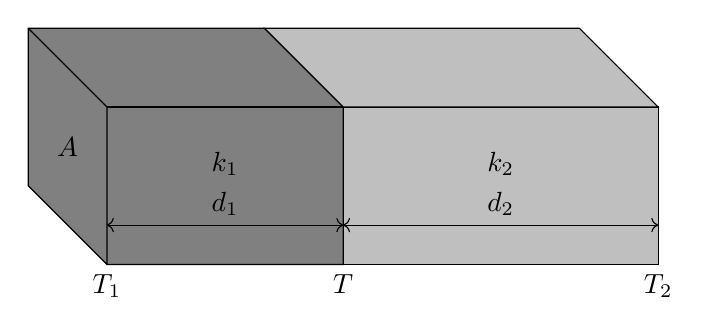
\begin{tikzpicture}
%\draw[step=1cm,gray,very thin] (0,0) grid (14,6);

\node[anchor=north, align=center] at (0,0) {$T_1$};
\node[anchor=north, align=center] at (3,0) {$T$};
\node[anchor=north, align=center] at (7,0) {$T_2$};

%\draw[fill=gray](0,0) rectangle (3,2);
%\draw[fill=gray](0,0) -- (-1,1) -- (-1,3) -- (2,3) -- (3, 2) -- (0, 2) -- (0,0) -- cycle;

%\draw[fill=gray](0,0) -- (3,0) -- (3,2) -- (2,3) -- (-1,3) -- (-1,1) -- (0,0) -- (0,2) -- (-1,3) -- (0,2) -- (3,2) -- (0,2);


\draw[fill=gray] (0,0) -- (-1,1) -- (-1,3) -- (2,3) -- (3,2) -- (3,0) -- (0,0) -- (0,2);

\draw(-1,3) -- (0,2);

\draw(0,2) -- (3,2);

\draw[fill=lightgray](3,0) rectangle (7,2);
\draw[fill=lightgray](2,3) -- (6,3) -- (7,2) -- (3,2) -- (2,3) -- cycle;

\node[anchor=south, align=center] at (-0.5,1.25) {$A$};

\draw[<->](0,0.5) -- (3,0.5);
\node[anchor=south, align=center] at (1.5,0.5) {$d_1$};
\node[anchor=south, align=center] at (1.5,1) {$k_1$};

\draw[<->](3,0.5) -- (7,0.5);
\node[anchor=south, align=center] at (5,0.5) {$d_2$};
\node[anchor=south, align=center] at (5,1) {$k_2$};

\end{tikzpicture}
\end{center}

Given $n$ slabs placed in series, with the leftmost temperature begin $T_1$ and rightmost temperature $T_2$, the equivalent conductivity of the system of slabs is given by:

\[
\boxed{
k_{eq} = \frac{\sum_{i=1}^n d_i}{\sum_{i=1}^n \frac{d_i}{k_i}}
}
\text{ With two slabs, }
\boxed{
k_{eq} = \frac{d_1 + d_2}{\left(\frac{d_1}{k_1}\right) + \left(\frac{d_2}{k_2}\right)}
}
\]

When there are two slabs, the interface temperature $T$ is given by:

\[
\boxed{
T = \frac{\frac{k_1 T_1}{d_1} + \frac{k_2 T_2}{d_2}}{\frac{k_1}{d_1} + \frac{k_2}{d_2}}
}
\]

\subsubsection{Slabs in parallel}

\begin{center}
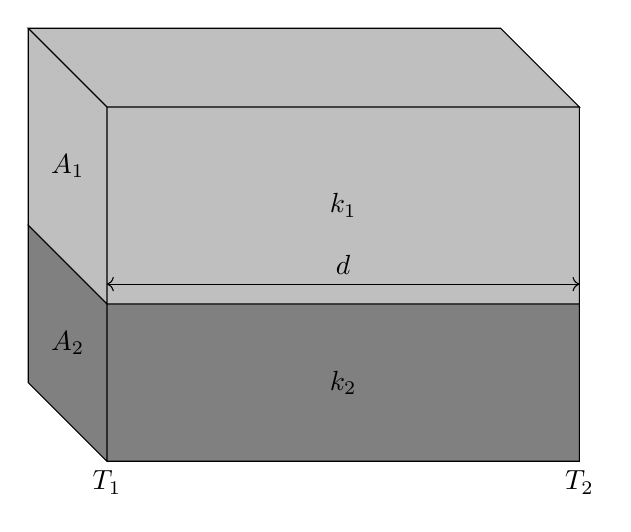
\begin{tikzpicture}
%\draw[step=1cm,gray,very thin] (0,0) grid (14,6);

\node[anchor=north, align=center] at (1,0) {$T_1$};
\node[anchor=north, align=center] at (7,0) {$T_2$};

\draw[fill=gray](1,0) -- (7,0) -- (7,2) -- (1,2) -- (1,0) -- (1,2) -- (0,3) -- (0,1) -- (1,0) -- cycle;
\node[anchor=center, align=center] at (0.5,1.5) {$A_2$};
\node[anchor=center, align=center] at (4,1) {$k_2$};

%\draw[fill=lightgray](0,6) -- (0,3) -- (1,2) -- (1,5) -- (1,2) -- (7,2) -- (7,5) -- (1, 5) -- (0, 6) -- (6,6) -- (7,5) -- (1,5);

\draw[fill=lightgray](0,5.5) -- (0,3) -- (1,2) -- (1,4.5) -- (1,2) -- (7,2) -- (7,4.5) -- (1,4.5) -- (0,5.5) -- (6,5.5) -- (7,4.5) -- (1,4.5);

%\node[anchor=center, align=center] at (0.5,4) {$A_1$};
\node[anchor=center, align=center] at (0.5,3.75) {$A_1$};
\node[anchor=center, align=center] at (4,3.25) {$k_1$};

\draw[<->](1,2.25) -- (7,2.25);
\node[anchor=south, align=center] at (4,2.25) {$d$};

\end{tikzpicture}
\end{center}

The rate of flow of heat in a system of $n$ parallel slabs:

\[
\boxed{
-\frac{\mathrm{d}Q}{\mathrm{d}t}=\frac{T_1 - T_2}{d}\sum_{i=1}^n k_i A_i
}
\]

The equivalent thermal conductivity of the system of parallel slabs:

\[
\boxed{
k_{eq} = \frac{\sum k_i A_i}{\sum A_i}
}
\]

\subsection{Newton's law of cooling for convection}

Given a mean temperature of $\theta$, a room temperature of $\theta_0$ and a constant $C$:

\[
\boxed{
-\frac{\mathrm{d}\theta}{\mathrm{d}t} = C(\theta - \theta_0)
}
\]

\subsection{Stefan-Boltzmann formula for radiation}

Given a radiator of area $A$, an absolute temperature $T_1$ of the radiator, a surrounding absolute temperature of $T_2$ and the Stefan-Boltzmann constant $\sigma$:

\[
\boxed{
- \frac{\mathrm{d}E}{\mathrm{d}t} = \sigma A \left(T_1^4 - T_2^4\right)
}
\]

\subsection{Wien's law for blackbody radiation}

Given the maximumx-intensity wavelength of blackbody radiation $\lambda_m$ at absolute temperature $T$:

\[
\boxed{
\lambda_m T = b = 4 \times 10^{-3} m\cdot K
}
\]

%The wavelength for maximum intensity of blackbody radiation is inversely proportional to the absolute temperature of the body.

\newpage

\subsection{Gas properties}

\subsubsection{Ideal gas law}

The ideal gas law states that in an ideal gas, given pressure $P$ in Pascal ($\frac{\text{N}}{\text{m}}$, volume $V$, amount of substance $n$ (in moles), absolute temperature $T$ and the ideal gas constant $R$ ($R=N_A \cdot k_b$, where Avagadro's constant $N_A = 6.022 \times 10^{23}$ and the Boltzmann constant $k_b = 1.381 \times 10^{-23}\text{J/K}$):

\[
\boxed{
PV = nRT
}
\]

By stating $k_b = R/N_A$ and number of molecules $N = n\cdot N_A$, ideal gas law is restated as:

\[
\boxed{
PV = NkT
}
\]

\subsubsection{Gas density}

Given a particuler gas with density $\rho$, pressure $P$ and absolute temperature $T$:

\[
\boxed{
\frac{\rho_1 T_1}{P_1} = \frac{\rho_2 T_2}{P_2}
}
\]

\subsubsection{Gas velocities}

Most probable speed:

\[
\boxed{
v_p = \sqrt{\frac{2kT}{m}}
}
\]

Average speed:

\[
\boxed{
< v > = \sqrt{\frac{8kT}{\pi m}}
}
\]

Root-mean-square speed:

\[
\boxed{
\sqrt{< v^2 >} = \sqrt{\frac{8kT}{m}}
}
\]

\subsection{Internal energy}

Internal energy $U$, given the constant volume heat capacity $c_v$ and absolute temperature $T$:

\[
\boxed{
U = n c_v R T
}
\]

$c_v$ is $\frac{3}{2} R$ for monatomic gases, and $\frac{5}{2} R$ for diatomic gases.

\newpage

\subsubsection{Specific heats}

Specific heat varies with the conditions that the gas is in: the heat capacity of the gas in  a container that expands with heat (constant pressure) is often much higher than when it's heated in a closed container that doesn't expand (constant volume).

Constant volume specific heat is $c_v$, and constant pressure specific heat is $c_p$.
The heat capacity ratio $\gamma$, given $c_p$ and $c_v$:

\[
\boxed{
\gamma = \frac{c_p}{c_v}
}
\]

The heat capacity ratio $\gamma$ depends on the degrees of freedom $f$ of the molecules of a gas:

\[
\boxed{
\gamma = 1 + \frac{2}{f}
}
\]

This can be reversed as well, to determine degrees of freedom of a gas from the specific heat ratio:

\[
\boxed{
f = \frac{2}{\gamma - 1}
}
\]

For a monatomic gas with 2 degrees of freedom:

\[
\boxed{
\gamma_{monatomic} = \frac{5}{3}
}
\]

For a diatomic gas with 5 degrees of freedom at room temperature:

\[
\boxed{
\gamma_{diatomic} = \frac{7}{5}
}
\]

\subsection{First law of thermodynamics}

Given $\Delta Q$ is the change in heat, $W$ is the work done by the system in a process and $\Delta U$ is the change in internal energy of the system:

\[
\boxed{
\Delta Q = \Delta U + W
}
\]

Internal energy $U$ of a system tends to increase when energy is added as heat and tends to decrease if energy is lost as work done by the system.

\subsection{Entropy}

Change in entropy $\Delta S$, given a change in heat $\mathrm{d}Q$ and a temperature $T$:

\[
\boxed{
\Delta S = \int \frac{\mathrm{d}Q}{T}
}
\]

\newpage

\subsection{Thermodynamic processes}

\subsubsection{Isobaric}

In isobaric processes, \textbf{pressure} remains constant: $\Delta P = 0$. The work done by the system in an isobaric process is given by:

\[
\boxed{
W = \int P \mathrm{d}V = P(V_1 - V_2) = P\cdot \Delta V
}
\]

Using ideal gas law:

\[
\boxed{
W = P \cdot \Delta V = nR \Delta T
}
\]

\subsubsection{Isochoric}

In an isochoric process, \textbf{volume} remains constant. No pressure-volume work is done because the volume remains constant ($Q = P\cdot\Delta V$, $\Delta V = 0$). This means that any change in heat comes from change in internal energy ($\Delta Q = \Delta U$).

\subsubsection{Isothermal}

In an isothermal process, \textbf{temperature} remains constant. There will be no change in internal energy, so $\Delta Q = W$.

\[
\boxed{
W_{\text{env}} = nRT\ln\left(\frac{V_2}{V_1}\right)
}
\]

\subsubsection{Adiabatic}

In an adiabatic process, heat remains constant. This means that there will be no $\Delta Q$, and that $\mathrm{d}U = -\mathrm{d}W$.

\[
\boxed{
W = \frac{1}{\gamma - 1}(P_2 V_2 - P_1 V_1)
}
\]

%$\gamma = \frac{c_p}{c_v}$, the ratio of two specific heats.

For an ideal gas undergoing an adiabatic process (adiabatic expansion, etc.), it can also be shown that:

\[
\boxed{
PV^\gamma = \text{constant}
}
\]

\newpage

\subsection{Heat engines}

\subsubsection{Thermodynamic efficiency}

The efficiency $e$ of a cycle:

\[
e = \frac{\text{Work done by gas}}{\text{Heat put into system}} = \boxed{\frac{W}{Q_{in}}}
\]

\subsubsection{Carnot cycle}

The Carnot cycle is the ideal thermodynamic cycle: it consists of two isothermal processes and two adiabatic processes.
Given a hot resevoir temperature of $T_H$ and a cold resevoir temperature of $T_C$:

\[
\boxed{
e = 1 - \frac{T_C}{T_H} = 1 - \frac{Q_C}{Q_H}
}
\]

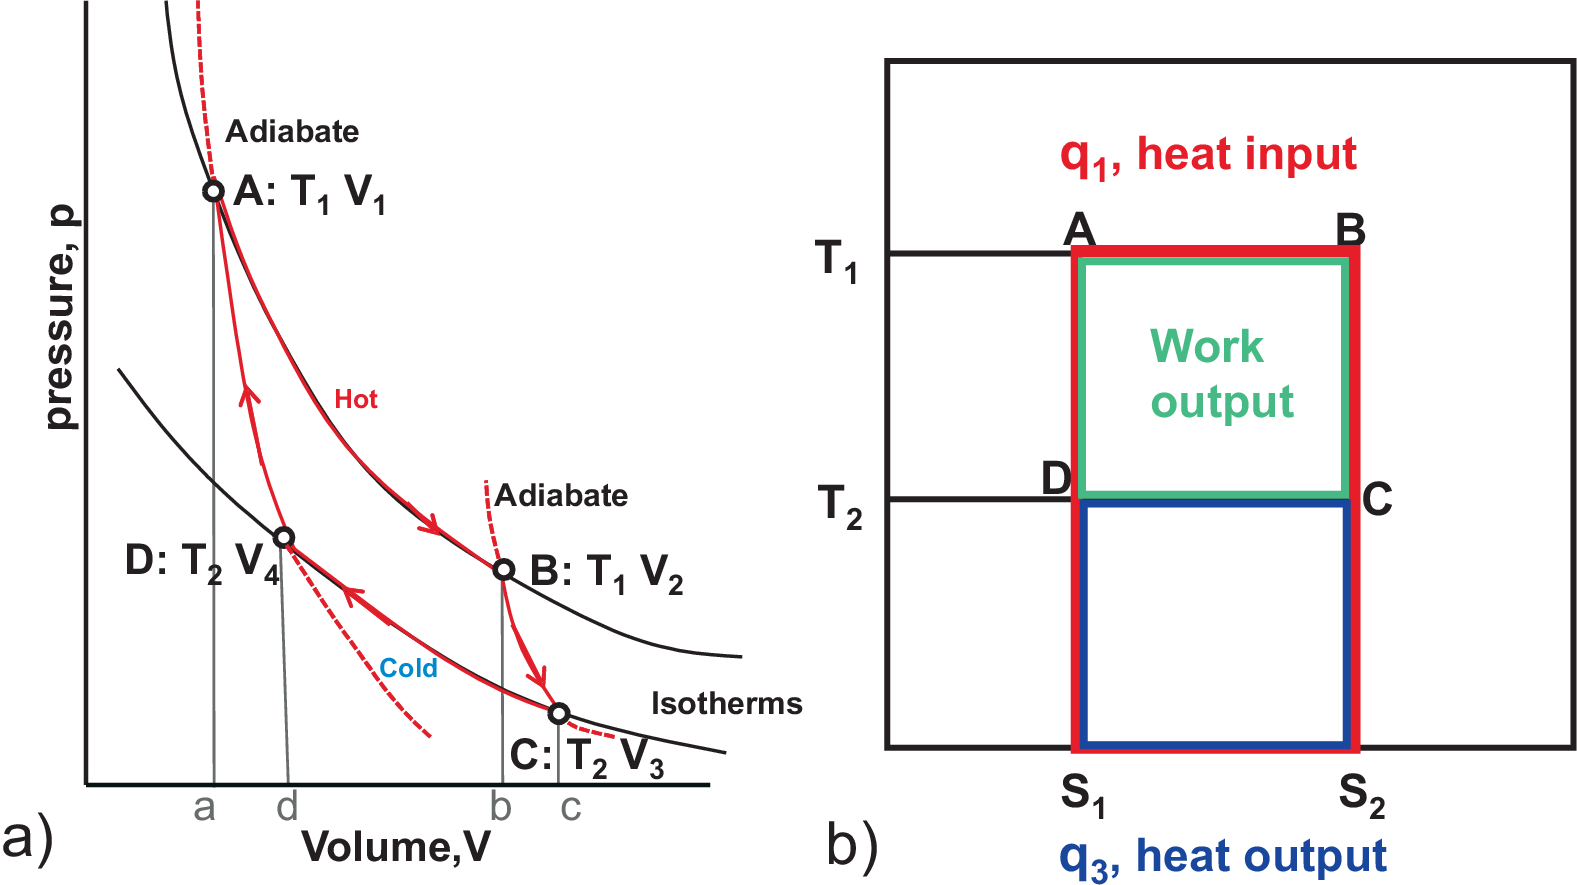
\includegraphics[width = 6.5in]{carnot_cycle_pv_ts.png}

$A \longrightarrow B$ and $C \longrightarrow D$ are isothermal processes, and $B \longrightarrow C$ and $D \longrightarrow A$ are adiabatic processes.
As $T_C$ is lowered and $T_H$ is raised, the efficiency of the heat engine increases.

\subsubsection{Sterling cycle}

The Sterling cycle consists of two isothermal processes and two isochoric processes.

\subsubsection{Otto cycle}

The Otto cycle consists of two adiabatic processes and two isochoric processes.

\newpage

\section{Material properties}

\subsection{Stress and strain}

Stress is applied force over an area.

\[
\boxed{
\text{Stress} = \frac{F}{A}
}
\]

Strain is the change in length over the original length.

\[
\boxed{
\text{Strain} = \frac{\Delta L}{L}
}
\]

\subsection{Young's modulus}

The Young's modulus $Y$, given the stress and strain:

\[
\boxed{
Y = \frac{\text{Stress}}{\text{Strain}} = \frac{FL}{A \Delta L}
}
\]

\subsection{Shear modulus}

The shear modulus $\eta$, given shear stress and shear strain ($\Delta x/y$):

\[
\boxed{
\eta = \frac{\text{Shear stress}}{\text{Shear strain}} = \frac{F y}{A \Delta x}
}
\]

\subsection{Bulk modulus}

Bulk modulus $K$ is related to the pressure increment with volume strain ($\Delta V/V$):

\[
\boxed{
K = \frac{\text{Pressure increment}}{\text{Volume strain}} = \frac{\Delta P}{- \Delta V/V}
}
\]

\subsection{Poisson's ratio}

Poisson's ratio relates transverse and axial strain to each other.
For example, if you strain som rubber by compressing it, it will tend to stretch axially.
Poisson's ratio $\sigma$ is related to the ration of lateral and longitudial strain:

\[
\boxed{
\sigma = -\frac{\text{strain}_{\text{transverse}}}{\text{strain}_{\text{axial}}}
}
\]

\newpage

\subsection{Moduli relations}

The elastic moduli are related in various ways.

\[
\boxed{
Y = \frac{9 \eta K}{3K + \eta}
}
\]

\[
\boxed{
Y = 2 \eta (1 + \sigma)
}
\]

\[
\boxed{
Y = 3K(1 - 2\sigma)
}
\]

\[
\boxed{
\sigma = \frac{2K - 2\eta}{6K + 2\eta}
}
\]

\subsection{Radioactive decay law}

The probability per unit time that a nucleus will decay is a constant, independent of time.
That constant is the decay constant $\lambda$.

Given $N_0$ molecules with decay constant $\lambda$, the amount of molecules $N(t)$ is given by the radioactive decay law:

\[
\boxed{
N = N_0 e^{-\lambda t}
}
\]

\subsubsection{Half-life}

The half-life $T_{1/2}$ of a material is the amount of time it would take for half of the molecules in that material to decay.
This means that:

\[
\frac{N_0}{2} = N_0 e^{-\lambda T_{1/2}}
\]

\[
e^{-\lambda T_{1/2}} = \frac{1}{2}
\]

\[
-\lambda T_{1/2} = \ln\left(\frac{1}{2}\right) = -\ln\left(2\right)
\]

\[
\boxed{
\lambda = \frac{\ln(2)}{T_{1/2}} \approx \frac{0.693}{T_{1/2}}
}
\]

\newpage

\section{Waves}

\subsection{Universal wave equation}

Given the velocity of a wave $v$, its frequency $f$ and its wavelength $\lambda$:

\[
\boxed{
v = f\lambda
}
\]

\subsection{Basic wave equation}

Given a wave with amplitude $A$, wave number $k$, angular frequency $\omega$ and phase $\phi$:

\[
\boxed{
y(x,t) = A\sin(kx - \omega t + \phi)
}
\]

The wave number $k$ is related to the wavelength:

\[
\boxed{
k = \frac{2\pi}{\lambda}
}
\]

The wave number and angular frequency are related to the velocity of the wave:

\[
\boxed{
v = \frac{\omega}{k}
}
\]

%\subsection{Power of a sound}

\subsection{Intensity of a sound}

Given a sound source of power $P$ which is acting on an area $A$:

\[
\boxed{
I = \frac{P}{A} = \frac{P}{4\pi r^2}
}
\]

\subsubsection{Decibels and intensity measurement}

Soudn intensity is generally measured in units called decibels.
Decibels operate on a logarithmic scale, and the decibel level is referred to with $\beta$.

Given a sound of intensity $I$ compared to the reference intensity $I_0 = 10^{-12} \frac{W}{m^2}$:

\[
\boxed{
\beta = 10\log_{10}\left(\frac{I}{I_0}\right)
}
\]

This means that an increase of 10 decibels indicates a tenfold increase of intensity - a whole order of magnitude!

\newpage

\subsection{Simple harmonic motion}

Simple harmonic motion occurs when the restoring force is proportional to the displacement.

\[
\boxed{
\frac{\mathrm{d}^2 x}{\mathrm{d}t^2} = -\omega^2 x
}
\]

\subsection{Sound waves in pipes}

\subsubsection{Open pipes}

When a pipe is open at both ends, there will be antinodes at both ends of the pipe.

The fundamental wavelength $\lambda_1$ is related to the length of the pipe $L$:

\[
\boxed{
\lambda_1 = 2L
}
\]

The fundamental frequency can also be found from this.

\[
\boxed{
f_1 = \frac{v}{\lambda} = \frac{v}{2L}
}
\]

Higher harmonics will simply have multiples of the fundamental frequency.

\[
\boxed{
f_n = nf_1 = \frac{nv}{2L}\text{ for }n = 1,2,3...
}
\]

\[
\boxed{
\lambda_n = \frac{\lambda_1}{n} = \frac{2L}{n}\text{ for }n = 1,2,3...
}
\]

\subsubsection{Pipes closed on one end}

A pipe closed on one end will have a node on the closed end and an antinode on the open end.

The fundamental wavelength $\lambda_1$ is related to the length of the pipe $L$:

\[
\boxed{
\lambda_1 = 4L
}
\]

The fundamental frequency can also be found from this.

\[
\boxed{
f_1 = \frac{v}{\lambda} = \frac{v}{4L}
}
\]

Do note, however, that a pipe with one closed end will actually have no even harmonics: there will only be 1st, 3rd, 5th, 7th harmonics and so on.

\[
\boxed{
f_n = nf_1 = \frac{nv}{4L}\text{ for }n = 1,3,5...
}
\]

\[
\boxed{
\lambda_n = \frac{\lambda_1}{n} = \frac{4L}{n}\text{ for }n = 1,3,5...
}
\]

\subsection{Waves on a stretched wire}

\subsubsection{Wave speed}

A wave on a stretched wire will travel as a certain speed $v$, given that it has a tension of $F$ and a linear density $\mu$:

\[
\boxed{
v = \sqrt{\frac{F}{\mu}} = \sqrt{\frac{F}{\rho A}}
}
\]

\subsubsection{Frequency}

The fundamental frequency of the vibrations, given tension $F$, length $L$, linear density $\mu$:

\[
\boxed{
f_1 = \frac{v}{\lambda} = \frac{1}{2L} \sqrt{\frac{F}{\mu}} = \frac{1}{2L} \sqrt{\frac{F}{\rho A}}
}
\]

The frequency of the $N$th harmonic is a multiple of the fundamental frequency:

\[
\boxed{
f_N = \frac{v}{\lambda_N} = \frac{N}{2L} \sqrt{\frac{F}{\mu}} = \frac{N}{2L} \sqrt{\frac{F}{\rho A}}
}
\]

\subsection{Doppler effect}

If the source of waves of frequency $f$ is moving with velocity $v_s$, the observer is moving at $v_o$, and the speed of sound in air is $v$:

\[
\boxed{
f' = f \frac{v \pm v_o}{v \mp v_s}
}
\]

$v_o$ is positive for motion towards the sound source and negative for motion away from the sound source.
$v_s$ is negative for motion towards the observer and positive for motion away from the observer.

\newpage

\section{Fluids}

\subsection{Jargon}

\emph{Steady flow (laminar flow)} means that the velocity of the fluid at a point is always the same.

\emph{Irrotational flow} means that the elements of fluid at every single point have no net angular velocity about that point, and implies the absence of eddies and vortices in the flow.

\emph{Incompressible fluid flow} means that a liquid is incompressible if its density is constant.

\subsection{Continuity of flow}

Because of conservation of mass (nothing is created or destroyed), a steady flow has to have the same mass of fluid passing all sections in a stream or fluid per unit time.

Given points $1$ and $2$ in a fluid flow, where the fluid has $\rho_{1,2}$ and $v_{1,2}$, and the pipe has cross-sectional area $A_{1,2}$:

\[
\boxed{
\rho_1 A_1 v_1 = \rho_2 A_2 v_2
}
\]

\subsection{Bernoulli's equation}

For a steady, non-viscous, incompressible flow:

\[
\boxed{
\frac{P}{\rho} + gh + \frac{1}{2}v^2 = \text{constant}
}
\]

It can also be stated as:

\[
\boxed{
P + \rho g h + \frac{1}{2}\rho v^2 = \text{constant}
}
\]

Bernoulli's equation represents the conservation of energy: the first term represents potential energy per unit mass of the liquid due to pressure, the second term represents potential energy due to gravity (e.g. due to changes in height of a tube), and the third term represents kinetic energy per unit mass of the liquid.

\subsection{Torricelli's theorem}

If there is a tank filled with liquid and an orifice located on the side of the tank at a depth $h$ below the surface of the liquid, the velocity of emergence of the liquid (also known as the velocity of efflux) is:

\[
\boxed{
v = \sqrt{2gh}
}
\]

\newpage

\subsection{Reynold's number and stability}

The stability of a fluid flow is represented by the Reynold's number $R$.
For any liquid flowing through a pipe, there is a critical velocity where laminar flow suddenly changes into turblent flow.

Given a liquid of density $\rho$ and viscosity $\eta$ flowing at a velocity $v$ through a pipe of diameter $d$:

\[
\boxed{
R = \frac{\rho v d}{\eta}
}
\]

If $R < 2200$, the flow is considered steady. If $R = 2200$, the flow is considered unstable, and if $R > 2200$, the flow is usually considered turbulent.

\subsection{Poiseuille's method for determining viscosity}

The volume $V$ flowing per second of a liquid of viscosity $\eta$ through a tube of radius $a$ and length $L$ under pressure $P$:

\[
\boxed{
V = \frac{\pi P a^4}{8\eta L}
}
\]

\subsection{Drag force}

The drag force $F$ on a sphere of radius $r$ is dropped into a liquid of viscosity $\eta$ is proportional to the velocity of that object:

\[
\boxed{
F = 6 \pi \eta r v
}
\]

\subsubsection{Terminal velocity}

When a sphere of radius $r$ and density $\rho_0$ is dropped into an extensive liquid of density $\rho$ and viscosity $\eta$, it will eventually approach a terminal velocity $v_T$ due to the drag force and buoyant force:

\[
\boxed{
v_T = \frac{2gr^2}{9\eta}(\rho_0 - \rho)
}
\]

\end{document}
